\section*{Population}
A species which has continuous birth and death rate is called a population.
\section{Describe and solve the single species population model. Find the doubling/tripling time. Discuss the plausibility and stability conditions.(Malthusian)}

The rate of change of population is proportional to the present population. Mathematically:
\begin{align*}
    \frac{dN}{dt} &\propto N \\
    \frac{dN}{dt} &= k N \sidenote{1}
\end{align*}

where $k$ is the proportionality constant (growth/decay rate), which may be positive or negative.

Separating variables and integrating:
\begin{align*}
    \frac{dN}{N} &= k \, dt \\
    \ln N &= kt + C \\
    N &= e^{kt + C} = e^{C} \cdot e^{kt} \\
    N &= A e^{kt} \sidenote{2}
\end{align*}
where $A$ is constant.
Using initial condition $N = N_0$ at $t = 0$:
\begin{align*}
    N_0 &= A e^{k(0)} \implies A = N_0
\end{align*}

Substituting $A$ back into (2):
\begin{align*}
    N(t) &= N_0 e^{kt} \sidenote{3}
\end{align*}

\textbf{Doubling Time ($T_d$):}

When $t = T_d$, the population doubles, i.e., $N = 2N_0$:
\begin{align*}
    2N_0 &= N_0 e^{k T_d} \\
    e^{k T_d} &= 2 \\
    k T_d &= \ln 2 \\
    \implies T_d &= \frac{\ln 2}{k} \approx \frac{0.6931}{k} \sidenote{Doubling time}
\end{align*}

\textbf{Tripling Time ($T$):}

When $t = T$, the population triples, i.e., $N = 3N_0$:
\begin{align*}
    3N_0 &= N_0 e^{kT} \\
    e^{kT} &= 3 \\
    kT &= \ln 3 \\
    \implies T &= \frac{\ln 3}{k} \approx \frac{1.0986}{k} \sidenote{Tripling time}
\end{align*}

\textbf{Plausibility Discussion:}
\begin{align*}
    \text{i. } &\text{For large time } t \to \infty \text{ (with } k > 0\text{), } N(t) \to \infty\text{, which gives an absurd/unrealistic} \nonumber \\
    &\text{result due to limited real-world environmental resources.} \nonumber \\
    \text{ii. } &\text{If initial population } N_0 \text{ is extremely large, the model similarly predicts unrealistic} \nonumber \\
    &\text{unbounded exponential growth.} \nonumber
\end{align*}
We have:
\begin{align*}
    N(t) = N_0 e^{kt} \sidenote{3}
\end{align*}

From solution (3), we analyze stability based on the parameter $k$:

\begin{enumerate}
    \item \textbf{Case 1 ($k > 0$):} 
    \begin{align*}
        \lim_{t \to \infty} N(t) \to \infty
    \end{align*}
    In this case, the system is \textbf{unstable} due to unbounded growth.

    \item \textbf{Case 2 ($k = 0$):} 
    \begin{align*}
        N(t) = N_0 \quad \text{for all } t \to \infty
    \end{align*}
    In this case, the population remains constant, so it is \textbf{stable} (neutrally stable).

    \item \textbf{Case 3 ($k < 0$):} 
    \begin{align*}
        \lim_{t \to \infty} N(t) \to 0
    \end{align*}
    In this case, the population is \textbf{asymptotically stable} as it decays to zero.\\
    \\
\end{enumerate}
\begin{center}
    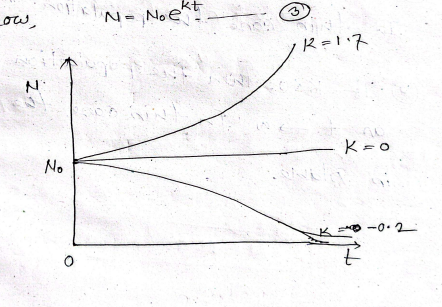
\includegraphics[]{Image/malthusian.png}
\end{center}